% Asset ID: A22StatisticalHypothesisTestingTIKZ-004
% Unit code: A22
% Topic code: A22-HT
% Topic name: Statistical hypothesis testing
% Related lesson section: Core Theory, Turning an exponential model into a straight-line model
% Source: Lesson transcript; Stats Yr2 Chapter 1 PDF; AS1 exponentials and logarithms support
% Purpose: Preserve the algebraic pathway from y = kb^x to log y = log k + x log b.
% Status: Phase 4 TikZ draft

\documentclass[tikz,border=8pt]{standalone}
\usepackage{amsmath}
\usepackage{tikz}
\usetikzlibrary{arrows.meta, positioning}
\begin{document}
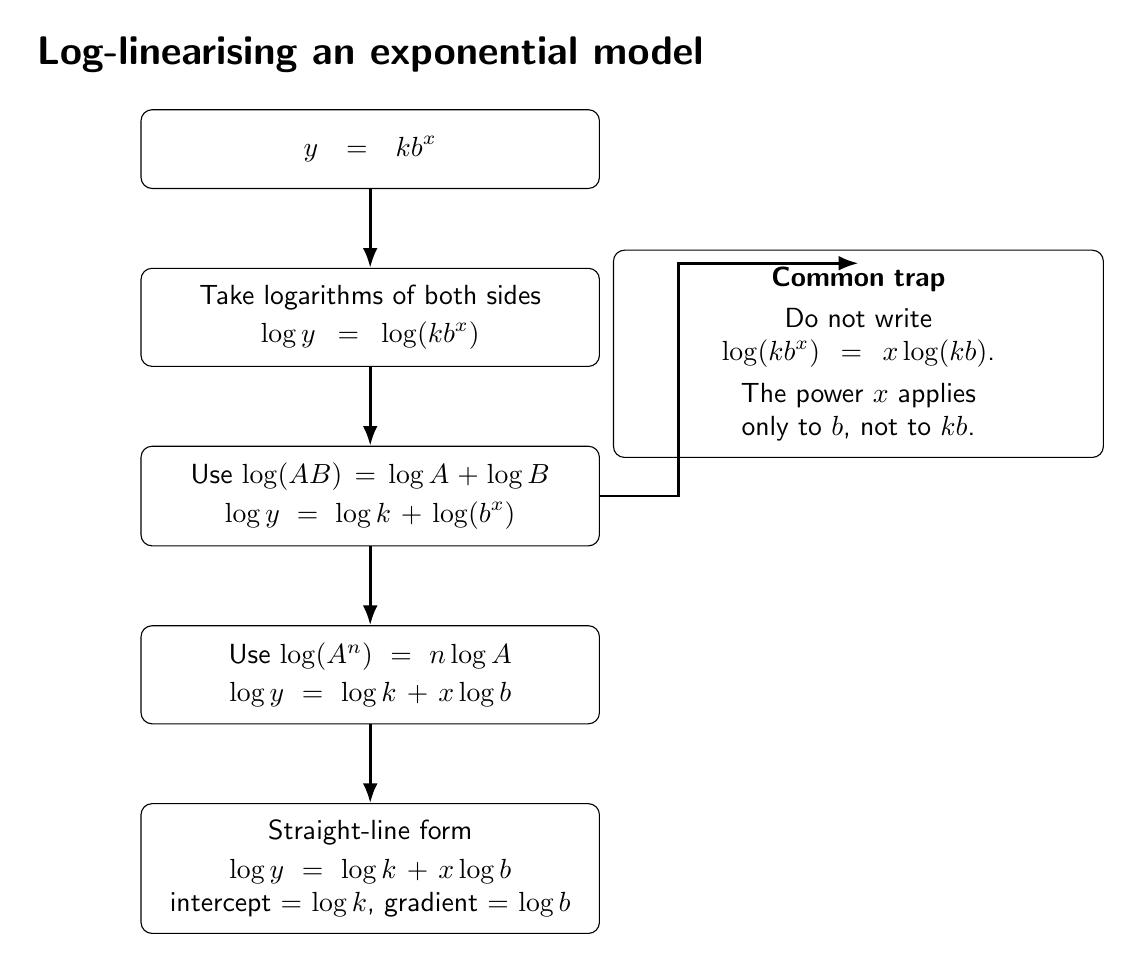
\begin{tikzpicture}[font=\sffamily,stepbox/.style={draw,rounded corners=4pt,align=center,text width=5.4cm,minimum height=1.0cm,inner sep=6pt},arrow/.style={line width=1pt,-{Latex[length=2.5mm]}}]
\node[font=\sffamily\bfseries\Large] at (0,4.4){Log-linearising an exponential model};
\node[stepbox] (s1) at (0,3.2){\(\displaystyle y=kb^x\)};
\node[stepbox, below=of s1] (s2){Take logarithms of both sides\\[2pt]\(\displaystyle \log y=\log(kb^x)\)};
\node[stepbox, below=of s2] (s3){Use \(\log(AB)=\log A+\log B\)\\[2pt]\(\displaystyle \log y=\log k+\log(b^x)\)};
\node[stepbox, below=of s3] (s4){Use \(\log(A^n)=n\log A\)\\[2pt]\(\displaystyle \log y=\log k+x\log b\)};
\node[stepbox, below=of s4] (s5){Straight-line form\\[2pt]\(\displaystyle \log y=\log k+x\log b\)\\intercept \(=\log k\), gradient \(=\log b\)};
\draw[arrow] (s1) -- (s2); \draw[arrow] (s2) -- (s3); \draw[arrow] (s3) -- (s4); \draw[arrow] (s4) -- (s5);
\node[draw,rounded corners=4pt,text width=5.8cm,align=center,inner sep=6pt] at (6.2,0.6){\textbf{Common trap}\\[3pt]Do not write\\\(\displaystyle \log(kb^x)=x\log(kb)\).\\[3pt]The power \(x\) applies only to \(b\), not to \(kb\).};
\draw[arrow] (s3.east) -- ++(1.0,0) |- (6.2,1.75);
\end{tikzpicture}
\end{document}
